
% VYSOKOŠKOLSKÁ KVALIFIKAČNÍ PRÁCE
% autor: Michal Struna
% název: Umělá inteligence pro detekci exoplanet

\documentclass[a4paper,12pt]{article}

\usepackage{utils}
\usepackage{titletoc}
\usepackage{amssymb}  % TODO: Odebrat
\usepackage{amsmath}

\def\code#1{\texttt{#1}}


\expandafter\def\expandafter\UrlBreaks\expandafter{\UrlBreaks%  save the current one
  \do\-}


% ÚDAJE O PRÁCI
\def\jmenoFakulty{Fakulta elektrotechniky a informatiky}
\def\jmenoAutora{Michal Struna}
%\def\nazevPrace{Umělá inteligence pro detekci exoplanet}
%\def\nazevPrace{Distribuované výpočty a umělá inteligence\\ pro detekci a analýzu exoplanet}
\def\nazevPrace{Detekce a~analýza exoplanet s~využitím\\distribuovaných výpočtů a~umělé inteligence}
\def\typPrace{Diplomová práce}
\def\rok{2021}
\def\prefixZadani{img/zadani}	% cesta a začátek jména, bude doplněno číslo strany
\def\suffixZadani{.jpg}		% doplní se ke každému jménu souboru zadání
\def\datumOdevzdaniPrace{9.\,5.\,2021}

\long\def\textPodekovani{...}


\long\def\anotace{
...
}
\def\klicovaSlova{exoplanety, extrasolární planety, kepler, umělá inteligence, python}
\def\title{Artificial intelligence for exoplanet detection from transit data}
\long\def\annotation{
...
}
\def\keywords{exoplanet, extrasolar planets, kepler, artificial intelligence, python}

%%%%%%%%%%%%%%%%%%%%%%%%%%%%%%%%%%%%%%%%%%%%%%%%%%%%%%%%%%%%
% ZAČÁTEK DOKUMENTU
%%%%%%%%%%%%%%%%%%%%%%%%%%%%%%%%%%%%%%%%%%%%%%%%%%%%%%%%%%%%

\begin{document}

\deskpage
\mainpage
\assignment
\statement
\acknowledgment
\annotationcs	
\annotationen
\content
\imglist
\tablelist
\codelist
\formulalist
\shortlist

\begin{description}[font=\mdseries,leftmargin=6em,labelwidth=!,]
\item[csv]      Comma-separated values
\item[fits]     Flexible image transport system
\item[ly]		Light year
\item[au]		Astronomical unit
\end{description}

\clearpage\pagestyle{plain}\phantomsection\addcontentsline{toc}{section}{Úvod}
\section*{Úvod}
\label{uvod}

První potvrzená planeta mimo sluneční soustavu byla objevena již roku 1992, ale výzkum exoplanet se dostal do oblasti širokého zájmu až během posledního desetiletí. Stalo se tak především kvůli vesmírnému teleskopu Kepler, který má na svém kontě od roku 2009 přes 2~500 objevených exoplanet.

K~dnešnímu dni je známo celkem více jak 4 000 potvrzených exoplanet. Toto číslo se s~nejvyšší pravděpodobností bude rychle zvyšovat, protože roku 2018 byl vypuštěn nástupce Kepleru -- satelit TESS -- od něhož je očekáván objev 20~000 exoplanet.

Planety u~jiných hvězd většinou nelze pozorovat přímo. Proto je nepřímými metodami zkoumáno jejich působení na své mateřské hvězdy, které už pozorovat lze. Výstupem z~takovýchto teleskopů jsou často stovky GiB nebo jednotky TiB fyzikálních a~statistických dat, jež je následně nutno zpracovat.

Cílem této diplomové práce je vytvořit aplikaci umožňující uživatelům poskytovat výpočetní výkon svých počítačů pro analyzování právě těchto dat. Projekt bude sestávat z~klientského konzolového programu, webové aplikace a~serveru. Klientský program bude provádět potřebné distribuovatelné výpočty na počítači uživatele. Tento program bude možné ovládat z~rozhraní webové aplikace, jež bude zároveň poskytovat přehled o~všech aktivitách, uživatelích a datech. Rozdělování výpočetních úloh mezi uživatele a~ukládání dat do databáze bude řešit server.

Díky distribuovaným výpočtům se do výzkumu exoplanet bude moci bez vysokého úsilí, znalosti či technického vybavení zapojit i široká veřejnost. To může urychlit vývoj a zároveň zvýšit povědomí o~této vědní disciplíně.

V~projektu jsou využity některé techniky spadající pod umělou inteligenci, v~důsledku čehož je zpracovávání dat zcela automatizované. Platí však, že umělá inteligence je v~současnosti stále intenzivně se rozvíjející oblastí, a~proto výsledky nemusí být natolik vypovídající ve srovnání s~tím, kdy by výzkum prováděli lidé manuálně, byť by to trvalo nesrovnatelně déle.

\section{Exoplanety}
\subsection{Důvody hledání}

TODO: Většina hvězd má planetu.

\subsection{Objevené exoplanety}

TODO: Statistické údaje, nejdůležitější exoplanety.

\subsection{Pojmenovávání exoplanet}

\section{Metody hledání exoplanet}

Exoplanety není téměř vůbec možné pozorovat přímo vizuálně, protože neemitují žádné světlo a~nachází se ve velkých vzdálenostech od Země. Lze ovšem pozorovat jejich působení na blízké hvězdy nebo jiné útvary, jež jsou pro nás viditelné. K~tomuto účelu se používá několik metod popsaných v této kapitole.

Zdaleka nejvýznamnější je tranzitní metoda, kterou byla objevena většina exoplanet. Velké množství planet bylo objeveno taktéž metodou radiálních vzdáleností. Pomocí ní byly objevovány planety především blízko Země.

\img[1]{Vlastnosti planet v závislosti na metodě objevení}{stats/count_by_method.pdf}

\dataplot

Málo hmotné planety byly objevovány jak tranzitní metodou, tak i~metodou radiálních rychlostí. Naproti tomu hmotné planety blízko své hvězdy byly objeveny především tranzitní metodou, kdežto hmotné planety daleko od své hvězdy metodou radiálních rychlostí. Nejvzdálenější planety od hvězdy byly pak objevovány metodou přímého zobrazení.

\img[1]{Závislost hmotnosti, periody oběhu a metody objevení planety}{stats/period_by_mass_by_method.pdf}

\dataplot

\clearpage
\subsection{Tranzitní metoda}

Někdy se planeta při obíhání dostane mezi svou hvězdu a~Zemi. Tento jev se pro pozorovatele na Zemi projeví jako mírný pokles jasu hvězdy (obvykle ve zlomku procenta). Pokud je hvězda teleskopem sledována dlouhodobě, je možné v~těchto změnách jasu hvězdy odhalit opakující se složku. To by mohlo indikovat přítomnost planety v~blízkosti této hvězdy.

\img[1]{Přechod planety přes kotouč hvězdy}{img/transit.png}
\drawgimp

Tyto změny však nemusí být na první pohled viditelné, protože v~soustavě může být více planet, které svou hvězdu zastiňují různou měrou a~obíhají kolem ní s~různou periodou. Navíc i v situaci, kdy je ve změnách jasu hvězdy objevena periodická složka nemusí jít vždy o~obíhající planetu. Hvězda může být např. sama o~sobě proměnlivá nebo se může jednat o~dvojhvězdu, jejíž složky se vzájmně zastiňují.

Tranzitní metoda vzbuzuje velký zájem především kvůli možnosti objevovat i~malé planety podobné Zemi~--~takové planety by mohly spíše splňovat podmínky pro život. Nevýhodou je, že pouze malé procento planet má dráhu v~rovině směrem k~pozorovateli na Zemi. Odhadem 97 \% \textbf{[TODO]} všech potenciálních planet nemůže být tranzitní metodou zachyceno.

\subsubsection{Target pixel file}

Prvním krokem v~analýze hvězdy tranzitní metodou je její fyzické pozorování. Teleskop obvykle pozoruje část oblohy po dobu několika měsíců, přičemž každých několik desítek minut vytvoří snímek dané části oblohy. Z~výsledných fotografií se následně vyextrahují jednotlivé hvězdy, čímž vzniknou tzv. target pixel files.

TPF obsahuje část oblohy o velikosti několika pixelů, na které se v původní fotografii nacházela zkoumaná hvězda a~její okolí. Barva pixelů je určena jasem.

\img[1]{Target pixel file hvězdy Kepler-10}{img/tpf.png}
\footnotetext[1]{Vytvořeno autorem v~Jupyter Notebook z~dat Kepleru od NASA}

\subsubsection{Světelná křivka hvězdy}

Po složení všech TPF do časové řady a~vypočítání jejich jasu dostaneme světelnou křivku. Na obrázku~5 je světelná křivka hvězdy Kepler-13 očištěná od dlouhodobého trendu, šumu a~extrémních hodnot. Křivka vykazuje velice výraznou periodickou složku s~periodou 1,763~dne. Ve většině případů ale vliv planety není takto výrazný a~detekovat planetu je obtížnější.

\img[1]{Světelná křivka soustavy Kepler-13}{img/light_curve.png}
\footnotetext[1]{Vytvořeno autorem.}

Každý tranzit má charakteristické fáze, které pomohou odlišit působení exoplanety od ostatních možných příčin, jako je např. proměnlivost hvězdy, dvojhvězda nebo pulzar.


\img[1]{Detail světelné křivky soustavy Kepler-13}{img/light_curve_detail.png}

\begin{enumerate}
\item Planeta je schovaná za hvězdou, hvězda je vidět se svým základním jasem.
\item Planeta je vedle hvězdy, jas hvězdy je posilněn o~světlo odražené od planety.
\item Planeta je vedle hvězdy, ale její viditelná část není osvětlena. Hvězda je vidět se svým základním jasem.
\item Planeta je před hvězdou, jas hvězdy je snížen v~důsledku zakrytí části kotouče.
\end{enumerate}

Tyto fáze společně s~důležitými parametry tranzitu potřebnými pro další výpočty jsou vyznačeny na obrázku~6:

\begin{enumerate}[label=\Alph*.]
\item Perioda -- čím větší perioda, tím delší planetární rok a větší velká poloosa dráhy,
\item Hloubka -- čím větší hloubka, tím je planeta vůči hvězdě větší,
\item Trvání -- čím je trvání kratší, tím menší trajektorii přes hvězdu planeta má,
\item Délka nástupu -- čím prudší a~kratší je nástup, tím menší je úhel mezi rovinou orbity exoplanety a~přímkou od hvězdy k~pozorovateli,
\item Délka minima -- čím větší délka minima v~porovnání s~délkou transitu, tím je úhel mezi rovinou orbity exoplanety a~přímkou od hvězdy k~pozorovateli menší.
\end{enumerate}

\subsubsection{Vyřazení false positives}

Většina periodických složek ve světelných křivkách hvězd jsou \emph{false positive}~--~patří jiným jevům, než je obíhající planeta. Tyto případy je třeba odfiltrovat, což byla až donedávna především manuální práce lidí -- vědců či dobrovolníků. Protože ale tranzit planety vykazuje specifický průběh popsaný v předchozí kapitole, je možné ho s~určitou úspěšností rozpoznat pomocí naučené umělé neuronové sítě automaticky.

\begin{multicols}{2}
\img[1]{Dvojhvězda KIC~8262223}{img/eclipsing_binary.png}
\img[1]{Cefeida KIC 3733346}{img/cepheid.png}
\end{multicols}

\begin{multicols}{2}
\img[1]{Proměnná hvězda KIC~9832227}{img/variable_star.png}
\img[1]{Kataklizmická proměnná hvězda KIC 9406652}{img/cataclysmic.png}
\end{multicols}

Je třeba aby vstupní data do neuronové sítě měla stejné rozměry i~formát. Vzhledem k~různorodosti světelných křivek je nutno provést několik kroků, abychom dosáhli standardizovaného formátu. Prvním krokem je složení časové řady do jedné periody, čímž dojde k~posílení viditelnosti transitu (pokud zde nějaký je), nebo naopak k~jeho vyrušení (pokud zde žádný není).

\pagebreak % TODO: Remove.

\begin{multicols}{2}
\img[1]{Světelná křivka Kepler-10}{img/full_light_curve.png}
\img[1]{Složená světelná křivka}{img/folded.png}
\end{multicols}

Na obrázku 12 je uprostřed slabě patrný transit. Má malou šířku, protože trvá pouze 0,25 dne, zatímco celá perioda je dlouhá 45,3 dne. Z~této složené časové řady se vytvoří dva pohledy, které budou vstupem do neuronové sítě:

\begin{itemize}
\item \textbf{Globální pohled} \emph{(obr. 13)} -- Šířka periody a~počet bodů v~časové řadě jsou fixní. Nevýhodou je, že u planet s~dlouhou periodou bude tranzit velice nepatrný, proto pouze globální pohled nestačí.
\item \textbf{Lokální pohled} \emph{(obr. 14)} -- Šířka tranzitu a počet bodů v časové řadě jsou fixní. Nevýhodou je, že není viditelný celý průběh světelné křivky. Naproti tomu je ale zřetelný tranzit.
\end{itemize}

\begin{multicols}{2}
\img[1]{Globální pohled na tranzit Kepler-10~c}{img/global_view.png}
\img[1]{Lokální pohled na tranzit Kepler-10~c}{img/local_view.png}
\nasa
\end{multicols}

Fixní počet bodů lze zajistit nahrazením každých $\frac{\alpha}{\beta}$ sousedních bodů ($\alpha$ -- současný počet bodů, $\beta$ -- požadovaný počet bodů) jediným, který bude reprezentovat jejich medián. Pro potřeby neuronové sítě je nutno oba pohledy taktéž normalizovat tak, aby platilo $H~=~\left<1; -1\right>$. U~případů, které neuronová síť vyhodnotí jako planety, je možné pokračovat výpočtem dalších informací o~planetě.

\subsubsection{Výpočet poloměru planety}

Ze světelné křivky a~poloměru hvězdy lze poloměr tranzitující planety vypočítat po vyjádření z~následující rovnice:

\formula{Poloměr planety z~tranzitní metody} {\frac{r^2}{R^2} = \frac{\Delta F}{F}}{
\begin{tabular}{llll}
	r = poloměr planety & R = poloměr hvězdy & F = jas hvězdy & $\Delta F$ = změna jasu \
\end{tabular}
}

\subsubsection{Výpočet hmotnosti planety}

Hmotnost planety z tranzitní metody narozdíl od metody radiálních rychlostí nelze vypočítat. Avšak z~empirických pozorování je možné hmotnost planety odhadnout z následující rovnice, přičemž $a$ a $b$ jsou pro různé velikostní kategorie jiné.

\formula{Odhad hmotnosti planety z~tranzitní metody} {m = a * r^b}{
\begin{tabular}{ll}
	m = hmotnost planety [hmotnost Země] & r = poloměr planety [poloměr Země] \
\end{tabular}
}

{
\tab{Odhad hmotnosti planety z~trantizní metody}{
	\begin{tabular}{|l|l|}
		\hline	
		\rowcolor{lightgray}
		Poloměr [poloměr Země] & Odhad hmotnosti \\	
		\hline	
		< 6 & $m = 0.9515 * r^{3.1}$  \\
		\hline	
		6-10 & $m = 1.7013 * r^{2.0383}$  \\
		\hline	
		10 > & $m = 0.6631 * r^{2.4191}$  \\
		\hline	
	\end{tabular}
}


\clearpage
\subsection{Metoda radiálních rychlostí}

Stejně jako hvězda ovlivňuje obíhající planetu, tak i~planeta gravitačně ovlivňuje svou hvězdu a~obě tělesa obíhají kolem společného těžiště. Tento pohyb se může projevit jako opakované přibližování a~vzdálování hvězdy vůči pozorovateli na Zemi. Právě pojem radiální rychlost označuje rychlost pohybu ve směru přímky k~pozorovateli.~\cite{methods}

Pokud se zdroj elektromagnetického záření (hvězda) přibližuje vůči pozorovateli, záření má menší vlnovou délku a~jeví se více do modra, protože právě modrá (a~fialová) barva má z~viditelného spektra nejmenší vlnovou délku. Obdobná situace nastává při vzdálování se zdroje vlnění od pozorovatele. Vlnová délka se zvětšuje a~barva jde do červena. Tomuto efektu se říká červený (resp. modrý) posuv.~\cite{methods}

\img[1]{Metoda radiálních vzdáleností}{img/radial_velocity.png}
\drawgimp

Zobecněním červeného posuvu je Dopplerův jev, který podobná pravidla vztahuje i~na jiné druhy vlnění (zvuk). Pokud se k~nám zdroj zvuku přibližuje (např. siréna na jedoucím autě), zvuk zpravidla vnímáme vyšším tónem, protože má menší vlnovou délku (vyšší frekvenci). Při vzdalování zdroje má zvuk větší vlnovou délku a je vnímán hlubším tónem. [TODO]

Periodicky se opakující změny ve vlnové délce záření hvězdy tak mohou být důsledkem existence tělesa v této soustavě.~\cite{methods}

\subsubsection{Měření vlnové délky záření hvězdy}

Hvězdy nevyzařují světlo pouze jedné jediné vlnové délky, nýbrž celé spektrum. Tento efekt lze vidět  u~duhy v~zemské atmosféře, kdy jsou jednotlivé složky slunečního světla odděleny. Záření z~hvězd se dokonce neomezuje pouze na viditelné světlo, ale pokrývá značnou část celého elektromagnetického spektra. Jak velká část záření přísluší jednotlivým vlnovým délkám lze měřit pomocí spektrometru.

\img[1]{Spektrum slunečního záření}{stats/sunlight_spectrum.png}
\footnotetext[1]{Vytvořeno autorem za využití datasetu \cite{sunlight}.}

Změna vlnové délky záření se projevuje jako horizontální posun barevného spektra hvězdy. Nutno podotknout, že zemská atmosféra některé vlnové délky pohlcuje. Proto i~přesto, že Slunce má barvu spíše do zelena vidíme tuto hvězdu ze Země žlutě.

\subsubsection{Výpočet radiální rychlosti hvězdy}

Poté, co teleskop sesbírá dostatečně velkou časovou řadu vlnových délek záření hvězdy může dojít k~vypočítání změn radiální rychlosti v~čase. Lze tak učinit dle vzorce~3. Platí, že radiální rychlost je kladná, pokud se zdroj od pozorovatele vzdaluje a~záporná pokud se přibližuje.

\formula{Radiální rychlost na základě změny vlnové délky} {v = c * \frac{\Delta\lambda}{\lambda_0}}{
\begin{tabular}{lll}
	$\Delta\lambda$ = změna vlnové délky & $\lambda_0$ = klidová vlnová délka & v = radiální rychlost \
\end{tabular}
}

Graf znázorňující radiální rychlost hvězdy 51~Pegasi může vypadat takto:

\img[1]{Radiální rychlost hvězdy 51 Pegasi}{stats/51_pegasi_radial_velocity.pdf}
\footnotetext[1]{Vytvořeno autorem za využití dat z~\cite{51pegasi}.}

Na první pohled je patrná jedna periodická složka s periodou 4,23 dne a~amplitudou 56,04 $\frac{m}{s}$, která značí, že kolem této hvězdy obíhá jedna planeta. Pokud zde jsou přítomna i~jiná tělesa, důvodů, proč je metoda radiálních rychlostí neodhalila může být několik:

\items{
\item Hmotnost tělesa je vůči hmotnosti hvězdy zanedbatelná,

\item Perioda oběhu tělesa je příliš velká (desítky let a~více), a~proto se ji nepodařilo zachytit na tak krátkém časovém úseku,

\item Těleso obíhá po dráze, jejíž rovina je kolmá k~přímce směrem~k pozorovateli (k Zemi). To vede k~tomu, že je hvězda vychylována takovým směrem, který nemá vliv na radiální rychlost hvězdy vůči Zemi.
}

V případě, kdy by kolem hvězdy obíhalo více planet by se průběh změn radiální rychlosti musel rozložit na jednotlivé složky stejně jako v~případě metody tranzitu v~grafu TODO.

\subsubsection{Výpočet údajů o~exoplanetě}

Z~pozorování hvězdy metodou radiálních vzdáleností lze získat mnohé informace o~planetě, která tuto hvězdu obíhá.

\items{
\item Perioda oběhu hvězdy T = perioda změn radiální rychlosti hvězdy,

\item Velká poloosa dráhy

\item Excentricita dráhy

\item Povrchová teplota planety

\item Minimální hmotnost planety $M_p$ lze odvodit z rovnice:

\formula[\cite{methods}]{Radiální rychlost}{\Delta v_{max} = \sqrt[3]{\frac{2\pi G}{T}} * \frac{M_p * sin(i)}{\sqrt[3]{(M_p + M_s)^2}} * \frac{1}{\sqrt{1 - e^2}}}{
\begin{tabular}{lll}
	$\Delta v_{max}$ = amplituda změny rychlosti & $M_s$ = hmotnost hvězdy & $M_p$ = hmotnost planety \\
	sin(i) = sklon dráhy vůči pozorovateli & e = excentricita dráhy & T = oběžná doba \\
\end{tabular}
}

}

Níže jsou uvedeny vlastnosti některých těles, na něž mohla být aplikována metoda radiálních vzdáleností. Ne všechna tělesa však byla touto metodou prvně objevena.

{ % TODO
\catcode`\-=12
\tab{Příklady údajů těles po aplikování metody radiálních vzdáleností}{
	\begin{tabular}{|l|l|l|l|l|l|l|l|}
		\hline	
		\rowcolor{lightgray}
		Těleso & Hvězda & $M_p$ [kg] & $M_s$ [kg] & sin(i) & e & T [r] & \textbf{$\Delta v_{max}$ [$\frac{m}{s}$]} \\	
		\hline	
		Země & \multirow{3}{*}{Slunce} & $5,97 * 10^{24}$ & \multirow{3}{*}{$2 * 10^{30}$} & \multirow{5}{*}{1} & 0,017 & 1 & \textbf{0,089} \\
		\cline{1-1}\cline{3-3}\cline{6-8}
		Jupiter & & $1,9 * 10^{27}$ & & & 0,048 & 11,86 & \textbf{12,4} \\
		\cline{1-1}\cline{3-3}\cline{6-8}
		\cline{1-1}\cline{3-3}\cline{6-8}
		Pluto & & $1,3 * 10^{22}$ & & & 0,247 & 247,41 & \textbf{0,00003} \\
		\cline{1-1}\cline{3-3}\cline{6-8}
		\cline{1-4}\cline{6-8}


		$\alpha$ Cen Bb & $\alpha$ Cen B & $6,75 * 10^{24}$ & $1,8 * 10^{30}$ & & 0 & 0,0089 & \textbf{0,51} \\	
		\cline{1-4}\cline{6-8}
		51 Pegasi b & 51 Pegasi & $0,88 * 10^{27}$ & $2,22 * 10^{30}$ & & 0,013 & 0,0116 & \textbf{55,9}  \\		
		\hline
	\end{tabular}
}

\clearpage
\subsection{Astrometrická metoda}

Astrometrická metoda využívá stejné vlastnosti vzájemného působení těles jako metoda radiálních rychlostí. Namísto zkoumání vlnové délky záření se však zaměřuje na polohu hvězdy. Hvězda, kolem níž obíhá dostatečně hmotné těleso, se bude v~důsledku působení tělesa nepatrně vychylovat ze své pozice~--~bude obíhat kolem těžiště soustavy.~\cite{methods}

\img[1]{Astrometrická metoda}{img/astrometry.png}

Pohyb hvězdy tak není přímočarý, ale vlnitý. Kolísání hvězdy je však pro pozorovatele na Zemi často pouze v~řádu stovek úhlových mikrovteřin až jednotek milivteřin.~\cite{methods} Z~tohoto důvodu byla astrometrickou metodou dosud objevena pouze jediná exoplaneta.~\cite{nasadata}

\img[1]{Kolísání hvězdy Gliese~876~s~planetou}{img/astrometry_trajectory.png}
\drawgimp

Dá se však očekávat, že se zlepšující se technikou bude tato metoda úspěšnější.

\tab{Ukázková tabulka}{
	\begin{tabular}{|l|l|c|c|c|c|c|c|}
		\hline	
		Data -0& Data 1& Data 2 & Data 3 & Data 4 & Data 5 \\
		\hline	
		Data 0& Data 1& Data 2 & Data 3 & Data 4 & Data 5 \\
		\hline	
		Data 0& Data 1& Data 2 & Data 3 & Data 4 & Data 5 \\
		\hline
	\end{tabular}
}

\lstinputlisting[caption={Spuštění programu}]{codes/usage.txt}

\subsection{Gravitační mikročočky}
\subsection{Přímé zobrazení}
\subsection{Pulsar timing}

\section{Umělá inteligence}

\subsection{Neuronová sít}

\subsubsection{Konvoluční neuronová síť}

\section{Použité technologie}

\subsection{TypeScript}

\subsubsection{React}

\subsubsection{Styled Components}

\subsubsection{NPM}

\subsection{Python}

\subsubsection{Flask}

\subsubsection{Astropy}

\subsubsection{LightKurve}

\subsubsection{TensorFlow}

\subsubsection{Pip}

\subsection{MongoDB}

\subsection{Socket.io}

\subsection{Git}


\section{Návrh~a~vývoj aplikace}

\img[1]{Komponenty projektu a~jejich komunikace}{img/communication.png}

\subsection{Server}

Úkolem serveru je přidělování výpočetních úloh připojeným klientským aplikacím, ukládání persistentních dat do databáze a~komunikace s~uživatelem skrze webovou aplikaci. Je naprogramován ve webovém frameworku Flask v~jazyce Python a~jeho adresářová struktura se dělí na následující moduly:

\img[1]{Architektura serveru}{img/server.png}
\draw

\begin{itemize}
\item \textbf{api} -- Definice REST a~Socket API a~zpracování příchozích požadavků. To zahrnuje autentizaci a~autorizaci odesílatele a~následné provedení operace v~servisní vrstvě. 
\item \textbf{config} -- Konfigurace serveru (např. připojení k~databázi). Základním konfiguračním souborem je \code{base.cfg}, který je použit automaticky. Bez nutnosti tento soubor měnit je možné vytvořit nový soubor (např. \code{test.cfg}) s~novou konfigurací a~pomocí argumentu při spuštění serveru nastavit, aby se použila tato konfigurace (\code{./src/main.py -{}-env test}). [TODO!!!]
\item \textbf{constants} -- Veškeré konstantní položky, ať už technického či fyzikálního typu.
\item \textbf{service} -- Servisní vrstva obsahující logiku serveru a~manipulaci s~databází.
\item \textbf{utils} -- Pomocné třídy uchovávající specifickou funkcionalitu.
\end{itemize}

\subsubsection{REST API}

K~vytvoření rozhraní je nejdříve třeba nadefinovat příslušné struktury, které rozhraní bude očekávat nebo naopak vracet. Modul \code{fields} umožňuje určit složky jednotlivých struktur a~taktéž pro ně nastavit pravidla jako např. maximální délka, datový typ nebo seznam povolených hodnot.

\lstinputlisting[caption={Vytvoření modelů v~REST API.}]{codes/api_model.txt}

Následně může dojit k~nadefinování koncových bodů rozhraní. Koncovým bodem jsou metody jakékoliv třídy, jež je potomkem \code{Resource}, přičemž názvy metod třídy odpovídají názvům metod HTTP.

\lstinputlisting[caption={Vytvoření koncového bodu v~REST API.}]{codes/rest_endpoint.txt}

Veškeré vstupní parametry od uživatele jsou automaticky parsovány, při nesprávnosti vstupních parametrů je odeslána chybová odpověď a~díky anotacím je také automaticky generována dokumentace REST API v~nástroji Swagger~UI dostupná na adrese \url{exoplanets.now.sh/api-docs}. Ukázka dokumentace REST API je umístěna v~příloze [TODO!!!] na konci dokumentu.

\subsubsection{Socket.io API}

Protože je třeba v~reálném čase synchronizovat webovou a~klientskou aplikaci a~umožnit serveru iniciovat s~těmito aplikacemi komunikaci, server kromě rozhraní HTTP poskytuje také rozhraní Socket.io.

\lstinputlisting[caption={Ukázka komunikace pomocí socket.io.}]{codes/socket.txt}

\subsection{Webová aplikace}

\img[1]{Architektura webové aplikace}{img/web_app.png}
\draw


\subsection{Klientská aplikace}

\img[1]{Stavy procesů a~přechody mezi nimi}{img/process_state.png}
\draw

\subsection{Neuronová síť}


\img[1]{Trénovací množina}{img/train_set.png}

\subsection{Databáze}

\subsection{Datasety}

Většina dat se do databáze nevkládá manuálně, jelikož je třeba pracovat se stovkami tisíc či miliony datových položkek. Namísto toho administrátor pouze definuje přístupový bod k~nějakému datasetu dostupnému přes webové rozhraní a~následně dojde k~automatickému zpracování datasetu a~všech položek v~něm. Některé typy datasetů jsou určeny k~jednorázovému uložení do databáze a~není nutno je nijak dál zpracovávat. Zpracování jiných je naopak výpočetně náročné a~připojené klientské aplikace postupně zpracovávají položku po položce. Jednotlivé typy datasetů jsou popsány níže.

U~všech typů datasetů je také vyřešena situace, kdy by se jedna a~ta samá položka (např. hvězda) nacházela ve dvou datasetech zároveň. V~takovém případě dojde k uložení obou hodnot a~uživatel v~aplikaci pak bude vidět údaje dané položky z~obou datasetů vedle sebe.

\subsubsection{Target pixel files}

\subsubsection{Světelné křivky hvězd}

\subsubsection{Radiální rychlosti hvězd}

\subsubsection{Hvězdy}

Informace o vlastnostech hvězd nejsou pro hledání exoplanet nutné, avšak pro spočítání dalších údajů o~nalezené exoplanetě je třeba je zahrnout do výpočtů. Datasety tohoto typu jsou k~dostání přes webová rozhraní nejčastěji ve formátu \code{csv}.

\img[1]{Část datasetu s~vlastnostmi hvězd}{img/star_properties.png}
\footnotetext[1]{Dataset pochází ze stránek \url{https://exoplanetarchive.ipac.caltech.edu}.}

Tyto datasety neobnáší žádné další složité výpočty, pouze jsou společně s dopočítanými údaji jednorázově uloženy do databáze. Základními údaji, které jsou pro každou hvězdu třeba, jsou (šedou barvou jsou dopočítané údaje):

\tab{Údaje o~hvězdách ukládané do databáze}{
    \begin{tabular}{|l|l|l|l|}
    \hline
    Název & Zdánlivá magnituda & Rovníkový průměr & \color{gray} Spektrální typ \\
    \hline
    Vzdálenost od Země & Hmotnost & \color{gray} Absolutní magnituda & \color{gray} Povrchová gravitace \\
    \hline
     Metalicita & Povrchová teplota & \color{gray} Průměrná hustota & \color{gray} Obyvatelná zóna \\
    \hline
    \end{tabular}
}

Aplikace je postavena flexibilně a~umožňuje libovolně namapovat sloupce z~datasetů do sloupců v~databázi. Datasety tak mohou mít pořadí i~názvy jednotlivých sloupců libovolné.


\subsubsection{Planety}

Datasety s~planetami nejsou pro běh aplikace taktéž nutné, protože veškeré informace o exoplanách jsou vypočítány z~jiných datasetů. Platí však, že čím více nezávislých zdrojů se na údajích o~exoplanetě shodne, tím spíše budou tyto údaje platné. Proto je umožněno ukládat do databáze i~datasety s~údaji o planetách -- mohou potvrdit nebo vyvrátit údaje vypočtené v~rámci aplikace.

\img[1]{Část datasetu s~vlastnostmi planet}{img/planet_properties.png}
\footnotetext[1]{Dataset pochází ze stránek \url{https://exoplanetarchive.ipac.caltech.edu}.}

Opět se jedná o~datasety nejčastěji ve formátu \code{csv}, které není nijak složitě zpracovávat, pouze uložit do databáze.

\tab{Údaje o~planetách ukládané do databáze}{
    \begin{tabular}{|l|l|l|l|}
    \hline
    Název & Povrchová teplota & Excentricita dráhy & Rovníkový průměr \\
    \hline
    Velká poloosa & Typ & Hmotnost & Perioda oběhu \\
    \hline
    Tranzit přes hvězdu & Průměrná hustota & Rychlost oběhu & Podmínky pro život \\
    \hline
    \end{tabular}
}

\subsubsection{Názvy}

Často se stává, že jedno a~to samé těleso je v~různých datasetech pod různým označením.

{
\tab{Pojmenování soustavy Kepler-10 v~různých katalozích TODO: Zdroj}{
	\begin{tabular}{|l|l|l|l|}
		\hline	
		\rowcolor{lightgray}
		Katalog & Účel & Označení Kepler-10 \\	
		\hline	
		KIC (\textbf{K}epler \textbf{I}nput \textbf{C}atalog) & Hledání exoplanet (Kepler) & KIC 11904151  \\
		\hline	
		KOI (\textbf{K}epler \textbf{O}bject of \textbf{I}nterest) & Výběr z~KIC & KOI-72  \\
		\hline	
		Kepler & Potvrzené exoplanety z~KOI & Kepler-10  \\
		\hline	
		2MASS (\textbf{2} \textbf{M}icron \textbf{A}ll-\textbf{S}ky \textbf{S}urvey) & Infra. průzkum oblohy & 2MASS J19024305+5014286  \\
		\hline		
		GSC (\textbf{G}uide \textbf{S}tar \textbf{C}atalog) & Pozorování hvězd (Hubble) & GSC 03549-00354  \\
		\hline
		Gaia DR (\textbf{G}aia \textbf{D}ata \textbf{R}elease) & Měření polohy hvězd (Gaia) & Gaia DR2 2132155017099178624 \\
		\hline
		USNO-B1.0 & Pozorování hvězd a~galaxií & USNO-B1.0 1402-00324696 \\
		\hline
		UCAC3 & Pozorování hvězd & UCAC3 281-142262 \\
		\hline
	\end{tabular}
}
\footnotetext[2]{Zdroj katalogů: \url{http://simbad.u-strasbg.fr/simbad/sim-id?Ident=Kepler-10}.}

K~zamezení toho, aby byly tyto položky vedeny jako dvě různé soustavy je nutno aplikaci poskytnout informace o~používaných názvech jednotlivých objektů. Právě k~tomu slouží tento typ datasetů.

\section{Rozvržení aplikace}

\subsection{Přehled}

\subsection{Databáze}

\subsection{Detail hvězdy}

\subsection{Detail planety}

\subsection{Objevování}

\subsection{Nápověda}

\subsection{Autentizace}

\section{Problémy řešené při implementaci}

\subsection{Virtualizace vykreslovaného seznamu}

Hvězdy i~detekované exoplanety jsou v aplikaci vykreslovány do tabulky. Z~praktických důvodů není tato tabulka rozdělena na stránky, mezi nimiž uživatel přepíná, ale je využita technika tzv. nekonečného scrollování (infinite scroll). Ta při načtení stránky zobrazí pouze několik prvních řádků a~teprve když uživatel doscrolluje dolů dojde k~načtení dalších několika řádků. Po dostatečně dlouhém scrollování tak může tabulka obsahovat velké množství řádků, jejichž vykreslování se negativně projeví na výkonu aplikace.

Z~tohoto důvodu je nutné, aby tabulka vykreslovala pouze ty řádky, které jsou viditelné a~nevykreslovala ty, jenž jsou mimo obrazovku. To povede k vykreslení vždy pouze několika řádků (v~závislosti na výšce řádků a~obrazovky) i~v~případě, kdy by tabulka obsahovala tisíce záznamů.


I~přesto, že pro JavaScript existují knihovny poskytující funkcionalitu virtualizovaného seznamu, žádná z~nich plně nevyhovuje potřebám aplikace, a~proto došklo k~vytvoření vlastní komponenty \code{VirtualizedList}.

\lstinputlisting[caption={Přiklad použití vlastní komponenty implementující virtualizovaný seznam}]{codes/virtualized_list.txt}

Komponenta si sama spočítá velikost obrazovky a~nutný počet vykreslovaných položek. Při scrollování dolů začne odebírat položky shora a~přidávat je dolů a~při scrollování nahoru naopak.

\img[1]{Porovnání klasického a~virtualizovaného seznamu}{img/virtualized_list.png}

\clearpage\pagestyle{plain}\phantomsection\addcontentsline{toc}{section}{Závěr}
\section*{Závěr}

\addcontentsline{toc}{section}{Použitá literatura}
\begin{thebibliography}{99}	% parametr určuje nejširší položku

\onlinesource{methods}{Metody objevování planet}{Astronomia}{23.~1.~2013}{~23.~12.~2019}{http://hvezdy.astro.cz/exoplanety/51-metody-objevovani-planet}

\onlinesource{nasadata}{NASA Exoplanet Archive}{NASA Exoplanet Science Insititute}{12.~8.~2019}{25.~12.~2019}{https://exoplanetarchive.ipac.caltech.edu/docs/API_exoplanet_columns.html}

\onlinesource[LOVIS, Christophe, FISCHER, Debra A]{radialvelocity}{Radial Velocity}{Yale Astronomy}{??.~?.~????}{25.~12.~2019}{http://exoplanets.astro.yale.edu/workshop/EPRV/Bibliography_files/Radial_Velocity.pdf}

\onlinesource{sunlight}{Reference Solar Spectral Irradiance: ASTM G-173}{nrel}{??.~?.~????}{27.~12.~2019}{https://rredc.nrel.gov/solar//spectra/am1.5/ASTMG173/ASTMG173.html}

\onlinesource{51pegasi}{The planet around 51 Pegasi}{The astrophysical journal}{1997}{29.~12.~2019}{https://iopscience.iop.org/article/10.1086/304088/pdf}

\end{thebibliography}

Exoplanets data \url{http://exoplanets.org/detail/alpha_Cen_B_b}

Wavelength \url{http://spiff.rit.edu/classes/phys240/lectures/expand/expand.html}

\clearpage\pagestyle{plain}\phantomsection\addcontentsline{toc}{section}{Seznam příloh}
\section*{Seznam příloh}

\noindent Příloha~A~~~~Architektura neuronové sítě \dotfill \pageref{priloha_a}

\section*{Příloha~A -- Architektura neuron. sítě}\label{priloha_a}
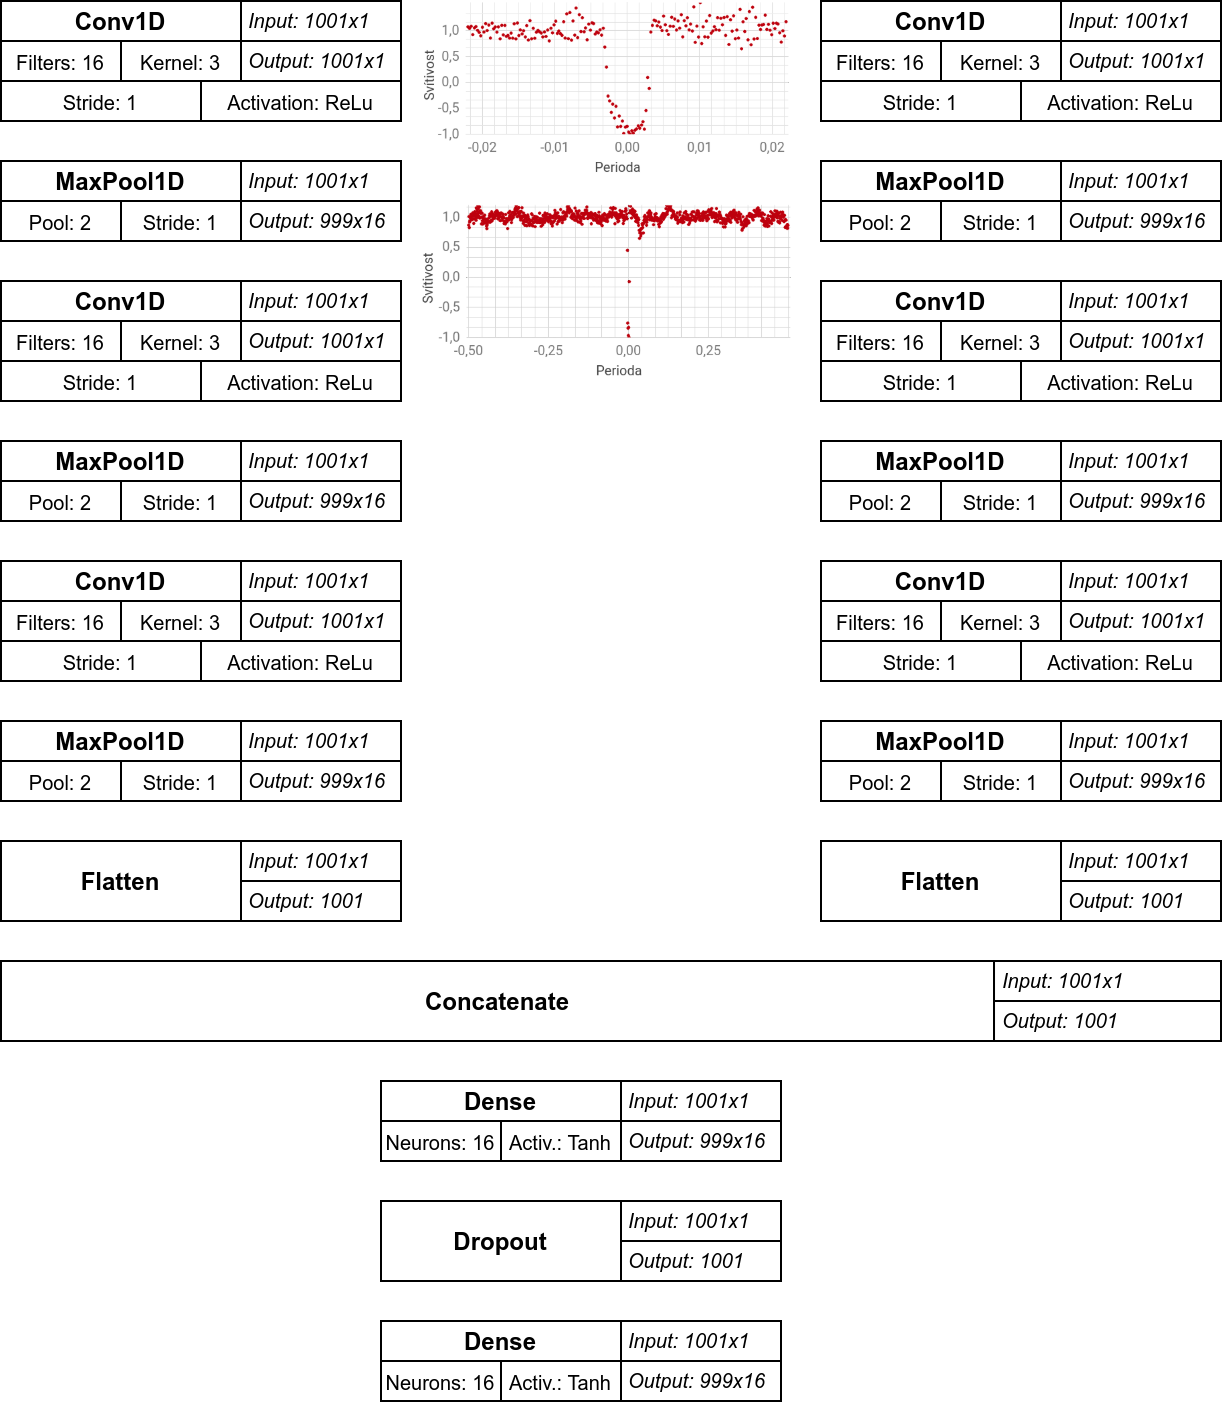
\includegraphics[width=\linewidth]{img/cnn.png}

\end{document}